%%=====================================================================
%%  5 系统模块设计与实现
%%=====================================================================
\section{系统模块设计与实现}

PMP 刷题系统的模块划分如图 \ref{fig:flowchart} 所示。

\begin{figure}[htbp]
  \centering
  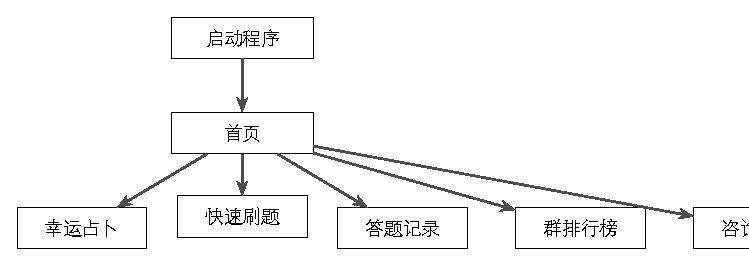
\includegraphics[width=0.80\textwidth]{figures/fig-flowchart.pdf}
  \caption{刷题系统模块流程图}
  \label{fig:flowchart}
\end{figure}

各模块的主要职责如下。

启动程序：进入微信小程序，程序自然启动。进入小程序后，主界面有 5 个模块，分别是幸运占卜、快速刷题、历史记录、群排行榜、咨询反馈。

首页：是整个小程序的门面，汇集五大模块。一般情况下，每次进入小程序最先进入首页。用户在首页可查看小程序的所有功能，从而进行相应的操作。同时，在幸运占卜模块右侧显示当前距离下一次 PMP 考试的天数。

幸运占卜：用户每次答题数满 20 题，可进行一次占卜。在这里用户可以抽取当日的幸运卡片，并将卡片分享至微信群或者将卡片保存至本地相册。

快速刷题：用户可以自己选择答题数量和答题章节进行快速刷题，用户答题完毕提交试卷后可自行选择继续答题还是查看答案解析。

群排行榜：用户可以将个人答题的得分分享至微信群，以及查看对应微信群中使用该小程序的用户的群排行榜得分情况。

答题记录：用户可以查看以往的答题记录，并且查看当时的题目解析。

咨询反馈：用户在使用过程中遇到问题，可以通过此模块进行留言反馈。

在功能实现方面，由于微信小程序 API 嵌套使用会导致代码过于繁琐冗长，且网络请求是异步的，而系统除咨询反馈以外的模块都需要检查登录状态再进行网络请求，因此本系统使用 Promise 和 Proxy 对网络请求和微信小程序的 API 进行了二次模块化封装，关键代码如下：

\begin{lstlisting}[style=js]
/* 对网络请求和自定义空 Promise 的封装 */
let services = {
  taskSequence: () => new Promise((resolve, reject) => { resolve(); }),
  httpClientPost: (url, data) => new Promise((resolve, reject) => {
    wx.request({
      url: url, data: data, method: 'POST',
      header: { 'Content-Type': 'application/json',
                'token': wx.getStorageSync('token') || '' },
      success: (res) => { resolve(res); },
      fail:    (res) => { reject(res);  },
    });
  }),
};

/* 对微信小程序的 API 通过 Proxy 进行二次封装 */
let wsAPI = new Proxy(services, {
  get: function (target, property) {
    if (property in target) { return target[property]; }
    else if (property in wx) {
      return (obj) => new Promise((resolve, reject) => {
        obj = obj || {};
        obj.success = (...args) => { resolve(...args); };
        obj.fail    = (...args) => { reject(...args);  };
        wx[property](obj);
      });
    }
  }
});
\end{lstlisting}

\subsection{首页界面设计与实现}

首页界面的布局主要采用了 MVVM 模式，建立数据模型，在 View 里面进行组件内容的显示，通过双向数据绑定来实现数据之间的交互。从主页跳转到其他页面通过调用 \texttt{wx.navigateTo} 或者 Navigator 组件实现，由于微信小程序的标签与 HTML 标签存在差异，所以无法通过 a 标签进行页面跳转。由于小程序的 Image 组件不支持使用本地图片，所以首页各模块的背景图片使用的是网络地址。

项目启动后，立即发出首页数据的网络请求，将请求获取到的数据解析并渲染到页面上。同时，对用户是否已经对小程序授权以及登录进行判断，若用户未授权，则弹出微信小程序系统授权框，引导用户授权使用小程序。

\subsection{快速刷题界面设计与实现}

快速刷题这个模块是答题系统的主要功能模块。具体实现：进入答题页面时，判断用户是否授权登录，若用户未授权则引导用户授权。然后将用户在首页选择的答题数量和答题章节通过网络请求发送给后台，从而获取到题目信息，并通过数据双向绑定的方式渲染答题界面。代码设计主要采用 MVVM 模式，通过代理模式请求网络通信和微信的 API，从而进行数据交互；通过封装的自定义模块显示 toast、modal 以及 loading；通过设置开关，避免用户多次点击造成数据的多次请求、渲染等问题。

用户提交试卷后，本次答题信息将通过网络请求传递给后台，后台接收参数进行一系列处理，将答案解析反馈回前端，用户可以选择继续答题或者查看答案解析。本次答题的正确率按式（\ref{equ:accuracy}）计算：

\begin{equation}
  P = \frac{N_{\mathrm{right}}}{N_{\mathrm{total}}} \times 100\%
  \label{equ:accuracy}
\end{equation}

式中：$P$ 为本次答题正确率；$N_{\mathrm{right}}$ 为答对题数；$N_{\mathrm{total}}$ 为本次答题总题数。

\subsection{群排行榜界面设计与实现}

群排行榜模块主要用于显示用户在不同的微信群中的排名情况。首次进入微信小程序的用户将小程序分享至一个或多个微信群中，才会获取到相对应的群组信息以及群成员排名信息。非首次进入小程序的用户，进入群组页面后会通过网络请求获取群组信息，再通过数据双向绑定渲染页面。

\subsection{答题记录界面设计与实现}

答题记录模块主要用于显示以往的答题记录，显示以往答题的正确率以及对应的试卷答案解析。这个界面可以采用上拉刷新加载更多，每一次上拉刷新都要请求一次服务器。上拉刷新实现的原理：每次上拉的时候请求服务器，服务器都会返回最新的第一页的数据，然后再把数据源添加到原数据数组的尾部，接着重新渲染当前页面，从而实现上拉刷新。

\subsection{咨询反馈界面设计与实现}

咨询反馈模块主要用于用户反馈小程序使用过程中遇到的问题，此模块不需要用户登录。用户提交留言后，会将用户反馈的信息以及用户机型等相关信息通过网络请求反馈给后台。

\subsection{幸运占卜界面设计与实现}

幸运占卜模块主要用于用户每日做题满 20 题后抽取当日幸运卡片。进入页面时会判断用户是否授权，若未授权则引导用户授权登录。若当日用户未做满 20 题，则显示眼睛特效——眼睛周围的图片根据重力感应可进行移动，点击蜡烛和眼睛都会播放对应的音效。用户在进入页面时会通过网络请求获取到本次抽签卡片的相关信息，并在用户抽签结束后渲染到卡片页面。用户可将抽取的卡片分享至微信群或将卡片保存在本地\cite{bib:qie}。
